\documentclass[]{article}
\usepackage[utf8]{inputenc}
\usepackage{lmodern}
\usepackage{mathtools}
\usepackage{amssymb}
\usepackage{theorem}
\usepackage{bm}

\topmargin=0cm
\textheight=700pt
\textwidth=430pt
\oddsidemargin=0pt
\headsep=0pt
\headheight=0pt 
\title{}
\author{Ozan, Ran}

\setlength{\parindent}{0pt}

\begin{document} 

\begin{flushright}
Ozan, Ran\\
\today\\
\end{flushright}

\centerline{ \Huge  \textbf{Applied Mathematics} }
\centerline{\Large  Home work 4}
\centerline{\Large  Face Recognition using PCA}
% % start of document.


\section*{ $\llcorner$  Chapter 1: Introduction $\urcorner$}

In this project, we implemented a face recognition system by using principal component analysis, which is known as $ PCA $. $ PCA $ method provide a mathematical way to reduce the dimension of problem. 
\\

Since the most elements of a facial image are highly correlated, it is better to extract a set of interesting and discriminative feature of a facial image. Mathematically speaking, we transform the correlated data to independent data. To implement the transform, we employed some linear algebra method such as SVD $ (Chapter 3) $. The main idea is to obtain $ Eigenfaces $ that every face can be regard as a linear combination of these eigenfaces $ (Chapter 4) $. Then the face recognition problem convert to a mathematic problem: what is the linear combination of a face? In other words, it simplify a problem from 2D to 1D.

\section*{ $\llcorner$  Chapter 2: Normalization $\urcorner$}
\subsection*{How to normalized images}
Normalization actually is a projection process. Because we detected the face images with different angle, we hope that we can use a same coordinate system for different angle faces. This coordinate system is a 64 $ \times $ 64 window which we predetermined five positions as facial features' location. These five locations is $ \overline{F} $. Once we have $ \overline{F} $, we can obtain affine transformation coefficients for each image as following figure shown. 
\begin{figure}[h]
\centering
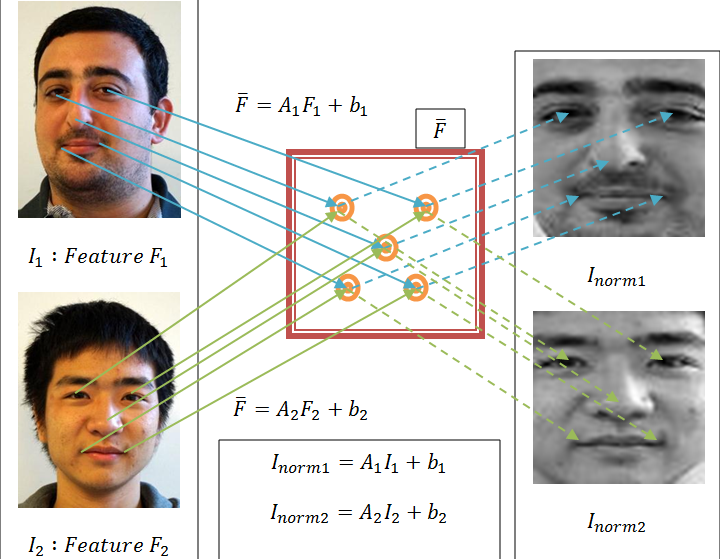
\includegraphics[width=0.7\linewidth]{./PCA1.png}
\caption{}
\end{figure}


In $ Figure 1 $, $ A_{i} $ and $ b_{i} $ are affine transformation matrix. Where $ A $ and $ b $ are given by:
$$
A = \begin{bmatrix} a_{11} & a_{12}\\ a_{21} & a_{22}\end{bmatrix} 
b = \begin{bmatrix} b_{1}\\ b_{2}\end{bmatrix} 
$$

\subsection*{How to compute A and b}

For each feature, the affine transformation is given by:
\begin{equation*}
f^{P}_{i} = Af_{i} + b
\end{equation*}
Where $ f_{i} $ is the feature location in original image and $ f^{P}_{i} $ is the position in normalization image. Since we already have $ f_{i} $ and $ f^{P}_{i} $ is also predetermined, let $ f = \begin{bmatrix} x\\ y\end{bmatrix} $, then the transformation can be written into:
\begin{equation*}
x^{P}_{i} = a_{11}x_{i} + a_{12}y_{i} + b_{1}
\end{equation*}
\begin{equation*}
y^{P}_{i} = a_{21}x_{i} + a_{22}y_{i} + b_{2}
\end{equation*}

We apply it on five features, the transformation is given by:
\begin{equation*}
 \begin{bmatrix} x1_{i} & y1_{i} & 1\\ x2_{i} & y2_{i} & 1\\ x3_{i} & y3_{i} & 1\\ x4_{i} & y4_{i} & 1\\ x5_{i} & y5_{i} & 1\end{bmatrix} 
 \begin{bmatrix} a_{11} & a_{21}\\ a_{12} & a_{22}\\ b_{1} & b_{2}\end{bmatrix} =  \begin{bmatrix} x1_{i}^{P} & y1_{i}^{P} \\ x2_{i}^{P} & y2_{i}^{P}\\ x3_{i}^{P} & y3_{i}^{P}\\ x4_{i}^{P} & y4_{i}^{P}\\ x5_{i}^{P} & y5_{i}^{P}\end{bmatrix} 
\end{equation*}
Until now, the problem convert to solve $ Ax=b $ in linear algebra. Since we got 10 equations for 6 unknowns, we employ SVD $( function \ pinv() \ in \ matlab )$ to solve it.

\subsection*{How to find $ \overline{F} $}
It is very important to get an appropriate $ \overline{F} $. We calculate $ \overline{F} $ by following steps:
\begin{itemize}
\item Step 1: We initialize $ \overline{F} $ with first image's feature to find average of all.
\item Step 2: Finding transformation that project $ \overline{F} $  to predefined position in 64x64 window. Then we can find this affine transformation as A and b matrices that has 6 parameters, and we apply this transformation to $ \overline{F} $.
\item Step 3: For each image feature $F_{i}$, we computing the A and b matrices for affine transformation that projecting  $ \overline{F} $ to $F_{i}$. 
\item Step 4: We change $ \overline{F} $ to averaged projected feature locations that we calculated previous step.
\item Step 5: If error between $ \overline{F}_{t} $ - $ \overline{F}_{t-1} $ is less than our threshold, we go back to step 2.
\end{itemize}

\section*{ $\llcorner$  Chapter 3: Principal Component Analysis $\urcorner$}
  We used PCA to transform our correlated data set into smaller uncorrelated data set. So PCA helped us on reducing the large dimensions of data set into smaller dimensions of it. After finding $ \overline{F} $, we followed these steps:\\
  \\
  We converted our 64 by 64 normalized images $X_{i}$  into row vector sized 1x4096 and constructed matrix $D_{pxd}$(p = number of images, d = 64x64) that each row corresponds to $X_{i}$. Then we defined k between 50 and 100 to \emph{k}th largest eigen values.\\
  \\Before computing the PCA, we computed the covariance matrix of D as follows:
  	$$ \Sigma = \frac{1}{p-1} D^{T} D $$
  	Then we used matlab's ``svd()" function to get eigenvectors from $ \Sigma $ matrix. This process in our training is taking the most time. We put k eigenvectors corresponding to biggest k eigenvalues to $\Phi$.
  	\\We calculated PCA space by;
  	$$ \phi_{i} = X_{i} . \Phi $$\\
  	
  	After all, now we can store all our training images in the PCA space and easily search them to find closest matches.
  

\section*{ $\llcorner$  Chapter 4: Recognition $\urcorner$}
blablabla...

\section*{ $\llcorner$  Chapter 5: Experimental Result and Analysis $\urcorner$}
We use No.1 and No.5 images of each person as test images and the rest are train images. For each test image, we calculate the distance of feature vector between test image and train images. Then we apply ascending sort on the train images by distance. Since we have three train images for each person, we shown top three of them.
\\

We are unable to get a ideal result which means three of them are matched, however it is acceptable if the first image is matched. We compute the accuracy which is the ratio of all results that first image is matched. The accuracy we got is 69.23$ \% $. Result of our matlab code shown by following figure.
\begin{figure}[h]
\centering
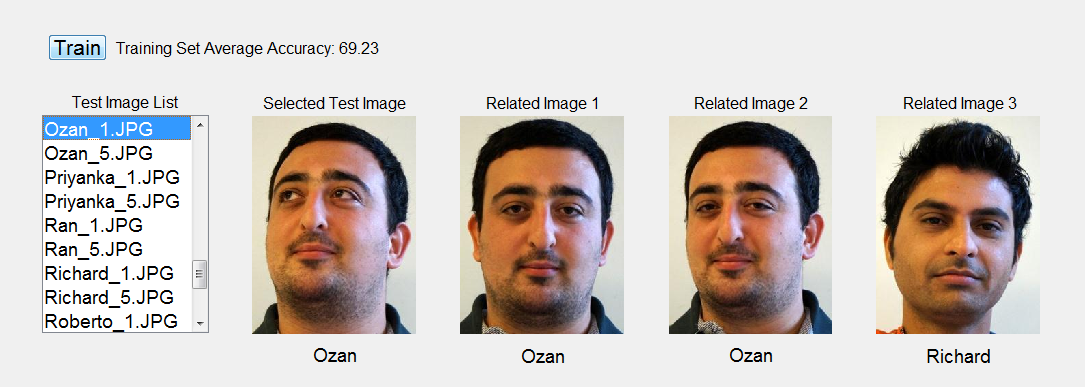
\includegraphics[width=0.7\linewidth]{./PCA2.png}
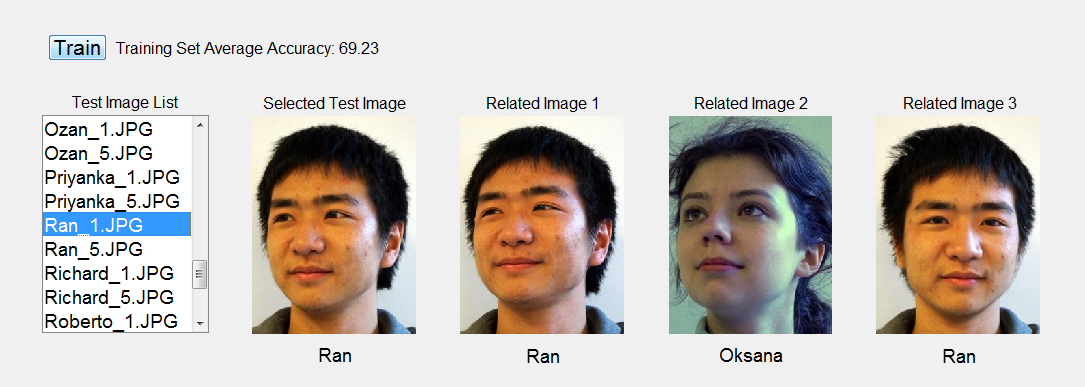
\includegraphics[width=0.7\linewidth]{./PCA4.png}
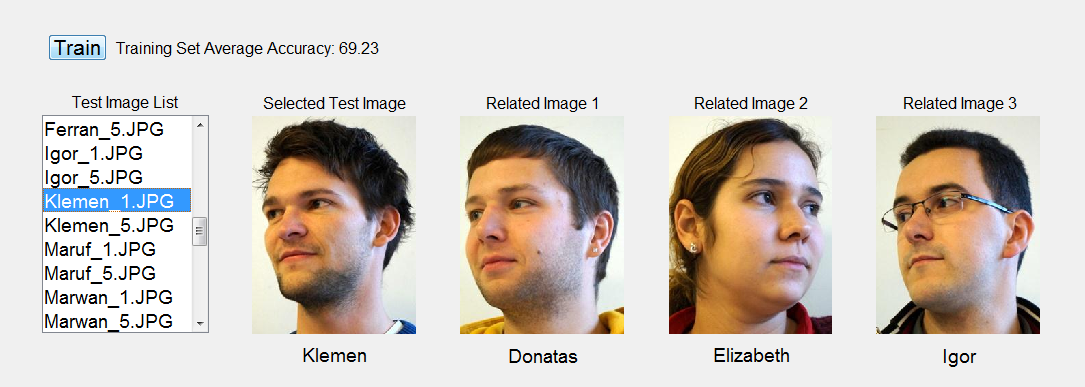
\includegraphics[width=0.7\linewidth]{./PCA5.png}
\caption{}
\end{figure}
\\

We also change the number of principal components $ (mark \ as \ k ) $. When $ k < 10 $, accuracy decrease effectively when we reduce $ k $. When $ k > 100 $, it has no effect on accuracy. In our finial result, we define $ k = 90 $.

\section*{ $\llcorner$  Chapter 6: Summary $\urcorner$}

This project help us understand a great idea that PCA provide: transform the data from correlated to independent. From image processing point of view, PCA is similar with Fourier transform which represent an image as the combination of some principal spectrum, Face recognition based on PCA actually represent a face by the combination of eigenfaces. It is a powerful method to reduce the dimension of problem.
\\

We also got some deeper understanding of the application of some linear algebra tools such as eigenvalue, eigenvector, SVD, etc. Specifically, we got the point that why and how we use SVD. 

\section*{ $\llcorner$  References $\urcorner$}

\end{document}
